%%% Preamble starts here.
\documentclass{amsart}
%for the heading
\usepackage{fancyhdr, enumerate}
%for the picture. 
\usepackage{tikz, calc}
%adjust the page width
\usepackage[margin=1in]{geometry}
\usepackage{float}


%% The next line says how the "vertex" style of nodes should look: drawn as small circles.
\tikzstyle{vertex}=[circle, draw, inner sep=0pt, minimum size=6pt]
%%
%% Next, we make a \vertex command as a shorthand in place of \node[vertex} to get that style.
\newcommand{\vertex}{\node[vertex]}

\linespread{1.1}


%special commands for number sets
\def\RR{{\mathbb R}}
\def\NN{{\mathbb N}}
\def\ZZ{{\mathbb Z}}
\def\QQ{{\mathbb Q}}
\def\CC{{\mathbb C}}
\def\WW{{\mathbb W}}
% header
\lhead{\sc  Senior Seminar: Homework 4}
\chead{\sc Stefano Fochesatto } 
\rhead{due: Friday 02/08/2020}
\cfoot{}
\pagestyle{fancy}

%%%% Main document starts here.

\begin{document}
\thispagestyle{fancy}
 
\begin{enumerate}
\item (Problem A) On page 22 of the text you will find a graph from Example 1.2.9. (On the page, the graph is between Example 1.2.9 and Remark 1.2.10.\\

Is the graph, $H,$ below a component of the graph from Example 1.2.9? Justify your answer. You answer must be formal and, therefore, it must use the definition of \emph{component}.

\begin{center}
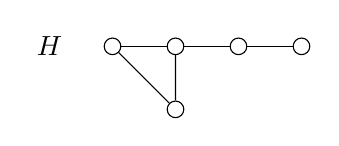
\begin{tikzpicture}[scale=.8] 
\node at (-1,1){$H$};
\vertex (t) at (1,0){};
\foreach \i in {0,1,2}{\draw (\i,1)--(\i+1,1);}
\foreach \i in {0,1,2,3}{\vertex[fill=white] (\i) at (\i,1){};}
\draw (0) -- (t)--(1);
\end{tikzpicture}
\end{center}

\textbf{Answer:} By definition the components of a graph $G$ are its maximal connected subgraphs. When we look at the graph $H$ above and compare it to the graph on page $22$ we can see that it is missing an edge and therefore it is not a maximal subgraph, because it could be made larger. 
	\vspace{0.25in}


\item (Problem B) Let $G_n$ be the graph with vertex set consisting of binary $n$-tuples. (So $V(G)=\{(a_1,a_2,\cdots,a_n) \: | \: a_i \in \{0,1\}\}.$) Two vertices of $G_n$ are adjacent if and only if the $n$-tuples differ in exactly two coordinates.\\
	\begin{enumerate}
	\item Draw $G_3.$\\
	\textbf{Answer:} Consider the following graph, Color coded by $n$-tuples that differ by exactly three coordinates.

\begin{figure}[H]
\caption{Graph $G_3$}
\centering
\includegraphics[width=.35\textwidth]{"g3graph".png}
\end{figure}
	
	\vspace{0.25in}
	
	\item For $v \in V(G_n),$ determine $\deg(v).$ (Justify your answer.)\\
	\textbf{Answer:} Consider vertex $v$. We can determine the number of vertices adjacent to $v$ by counting up the number of ways there is to change an arbitrary $n$-tuple by exactly two coordinates. Consider $n \choose 2$, since there are $n$ digits in the tuple and we are only choosing two of them to change. 
	
	\vspace{0.25in}
	
	\item Determine the number of components of $G_n.$ (Justify your answer.)\\
	\textbf{Answer:} In a $G_n$ there is always two components. Consider we partition the vertex set into two parts by if the number of ones that appear in the tuple are even or odd, ie $V_{E}(G_n)$ contains all even $n$-tuples and $V_{O}(G_n)$ contains all odd $n$-tuples. Consider vertices $u,v \in V_{E}(G_n)$ we know by the definition of the partition $V_{E}(G_n)$ that the $n$-tuples that represent $u$ and $v$ have a difference of $2k$ ones, where $k \in \WW$, and therefore there must exist a path between them in $G$. The same argument applies for vertices $u,v \in V_{O}(G_n)$. Now consider that vertex $u \in V_{E}(G_n)$ and $w \in V_{O}(G_n)$, by the definition of our parts we know that each $n$-tuple $u$ and $w$ differs by $2k+1$ ones, where $k \in \WW$. Therefore there cannot exist a path between them in $G$
	
	\vspace{0.25in}
	
	\end{enumerate}

\item (Problem 1.2.10) Prove or disprove:
	\begin{enumerate}
	\item Every Eulerian bipartite graph has an even number of edges.\\
	\textbf{Answer:} 
	
	
	
	
	
	 Suppose Eulerian bipartite graph $G$. From Theorem 1.2.26 we know that if a graph is Eulerian the degree of each vertex must be even. Since $G$ must be an even graph we know from Proposition 1.2.27 that $G$ decomposes into cycles. Since $G$ is a bipartite graph we know that it cannot contain an odd cycle from Theorem 1.2.18. Therefore $G$ is composed of even cycles and thus has an even number of edges. 
	
	\vspace{0.25in}
	
	\item Every Eulerian simple graph with an even number of vertices has an even number of edges.\\






	\textbf{Answer:} By counterexample. Consider the following graph. 
\begin{figure}[H]
\caption{Graph $H$}
\centering
\includegraphics[width=.5\textwidth]{"cycle5and4".png}
\end{figure}
 We can see that the graph has an odd number of edges and each vertex has an even degree. consider the Eulerian circuit $[A,D,C,D,A,E,F,G,A]$
	
	\vspace{0.25in}
	\end{enumerate}

\item (Problem 1.2.11) Prove or disprove: If $G$ is an Eulerian graph with edges $e$, $f$ that share a vertex, then $G$ has an Eulerian circuit in which $e$, $f$ appear consecutively.\\


	\textbf{Answer:} Consider Graph $H$ where edges $e$ and $f$ are labeled.\\
	\begin{figure}[H]
\caption{Graph $H$}
\centering
\includegraphics[width=.5\textwidth]{"cycle5and4labled".png}
\end{figure}
We showed that $H$ is Eulerian, and as we can see $e$ and $f$ share vertex $A$.
Note that, constructing a closed trail where edges $e$ and $f$ are consecutive will always result in a maximal trail that does not contain every edge in the graph $H$. Therefore there cannot exist an Eulerian circuit where $e$ and $f$ are consecutive. 

	\vspace{0.25in}

\item (Problem 1.2.25) Use ordinary induction on the number of edges or vertices to prove that the absence of odd cycles is a sufficient condition for a graph to be bipartite. 


	\textbf{Proof:} We will proceed by induction on the number of vertices$\ell$.

Base Case: Suppose Graph $G$ on $n$ vertices and has no odd cycles. Let $\ell = 0$. Note that every 2-partition of $V(G)$ is always disjoint, therefore $G$ is trivially bipartite.\\

Induction Hypotheses: Suppose a graph $G$ with no odd cycles, and $\ell$ edges is bipartite.\\

Induction Step: Suppose a graph $G$ with no odd cycles and $\ell+1$ edges. Consider an arbitrary edge $e$ in $G$ that is incident to vertices $u$ and $v$. Now consider $G-e$, we now have a graph with no odd cycles, $\ell$ edges. By the induction hypothesis $G-e$ is bipartite. Since $G-e$ is bipartite we can partition $V(G-e)$ into two disjoint sets such that no two vertices within the same set are adjacent. Note there will always exists a partition $V(G-e)$ where $u$ and $v$ are in different parts.  We can add edge $e$ back into the graph $G-e$ by selecting two vertices, one from each part. Thus we have shown that graph $G$ is bipartite. \\

	
	\vspace{0.25in}

\item (Problem C) Let $H$ be a connected graph with at least three vertices (so $u$, $x$ and $y$ are assumed to be distinct) and let $u$ be the endpoint of a maximal path in $H.$ Call this path $P.$ Let $x,y \in V(H)-u.$ Show that there exists an $xy$-path in $H-u.$

Case 1: $x$ and $y$ are inside of the path $P$. Since $P$ is a maximal path The neighbors of endpoint vertex $u$ must also lie on the path. Therefore when we delete $u$ we cannot disconnect the graph because all the neighbors of $u$ lie in $P$ and would therefore still be connected. Thus there must still exist an $xy$-path in $H-u.$ \\

Case 2: $x$ and $y$ are both outside of the path $P$. We know that $x$ and $y$ both are in a connected graph $H$ so there must exist an $xy$-path $Q$. Suppose $Q$ uses vertices from path $P$, we know that $Q$ cannot contain the endpoints of $P$ because then $P$ wouldn't be a maximal path. Therefore deleting an endpoint $u$ of path $P$ would not disrupt path $Q$. Now suppose $Q$ doesn't use vertices in $P$, then the deletion of vertex $u$ still wouldn't disrupt path $Q$. Thus $Q$ must still exist an $xy$-path in $H-u.$\\


Case 3: WLOG say that $x$ is contained in path $P$ and $y$ is not. Since $H$ is connected there must exist  $xy$-path $Q$. Note, in $Q$, If $x$ is directly incident to $u$ then path $P$ is no longer maximal. Therefore the first vertex in $Q$, from $P$ must be an inner vertex. and since that is the case there must always exist an $xy$-path that avoids using the endpoints of $P$. Thus there must still exist an $xy$-path in $H-u.$ \\\\\\


p.s. In the interest of transparency you should know that I worked with Brons for a majority of this homework, and I also helped Brett and Rohan approach the $n$ - tuple and Eulerian problems. 
\end{enumerate}
\end{document}



